% Pour faire une référence d'une annexe
% (Annexe \ref{sec:nomsection} page~\pageref{sec:nomsection})
\section{First appendix}
\label{sec:firstAppendix}
\begin{figure}[H]
	\centering
	% \includegraphics[keepaspectratio=true, width=0.7\textwidth]{Annexes/i/refletsDeLOmbreFantaisie.jpg}
	\caption{First appendix caption}
	\label{fig:firstAppendix}	
	\medskip
	\small
	\it
	Source quotation and descriptive text.
\end{figure}
\clearpage

% Appendix declaration with a 90° rotated figure
\rotatebox{90}{
	\begin{minipage}{0.90\textheight}
		\section{Modèle de l'application symbolist}
		\label{sec:symbolistModelClassDiagram}
		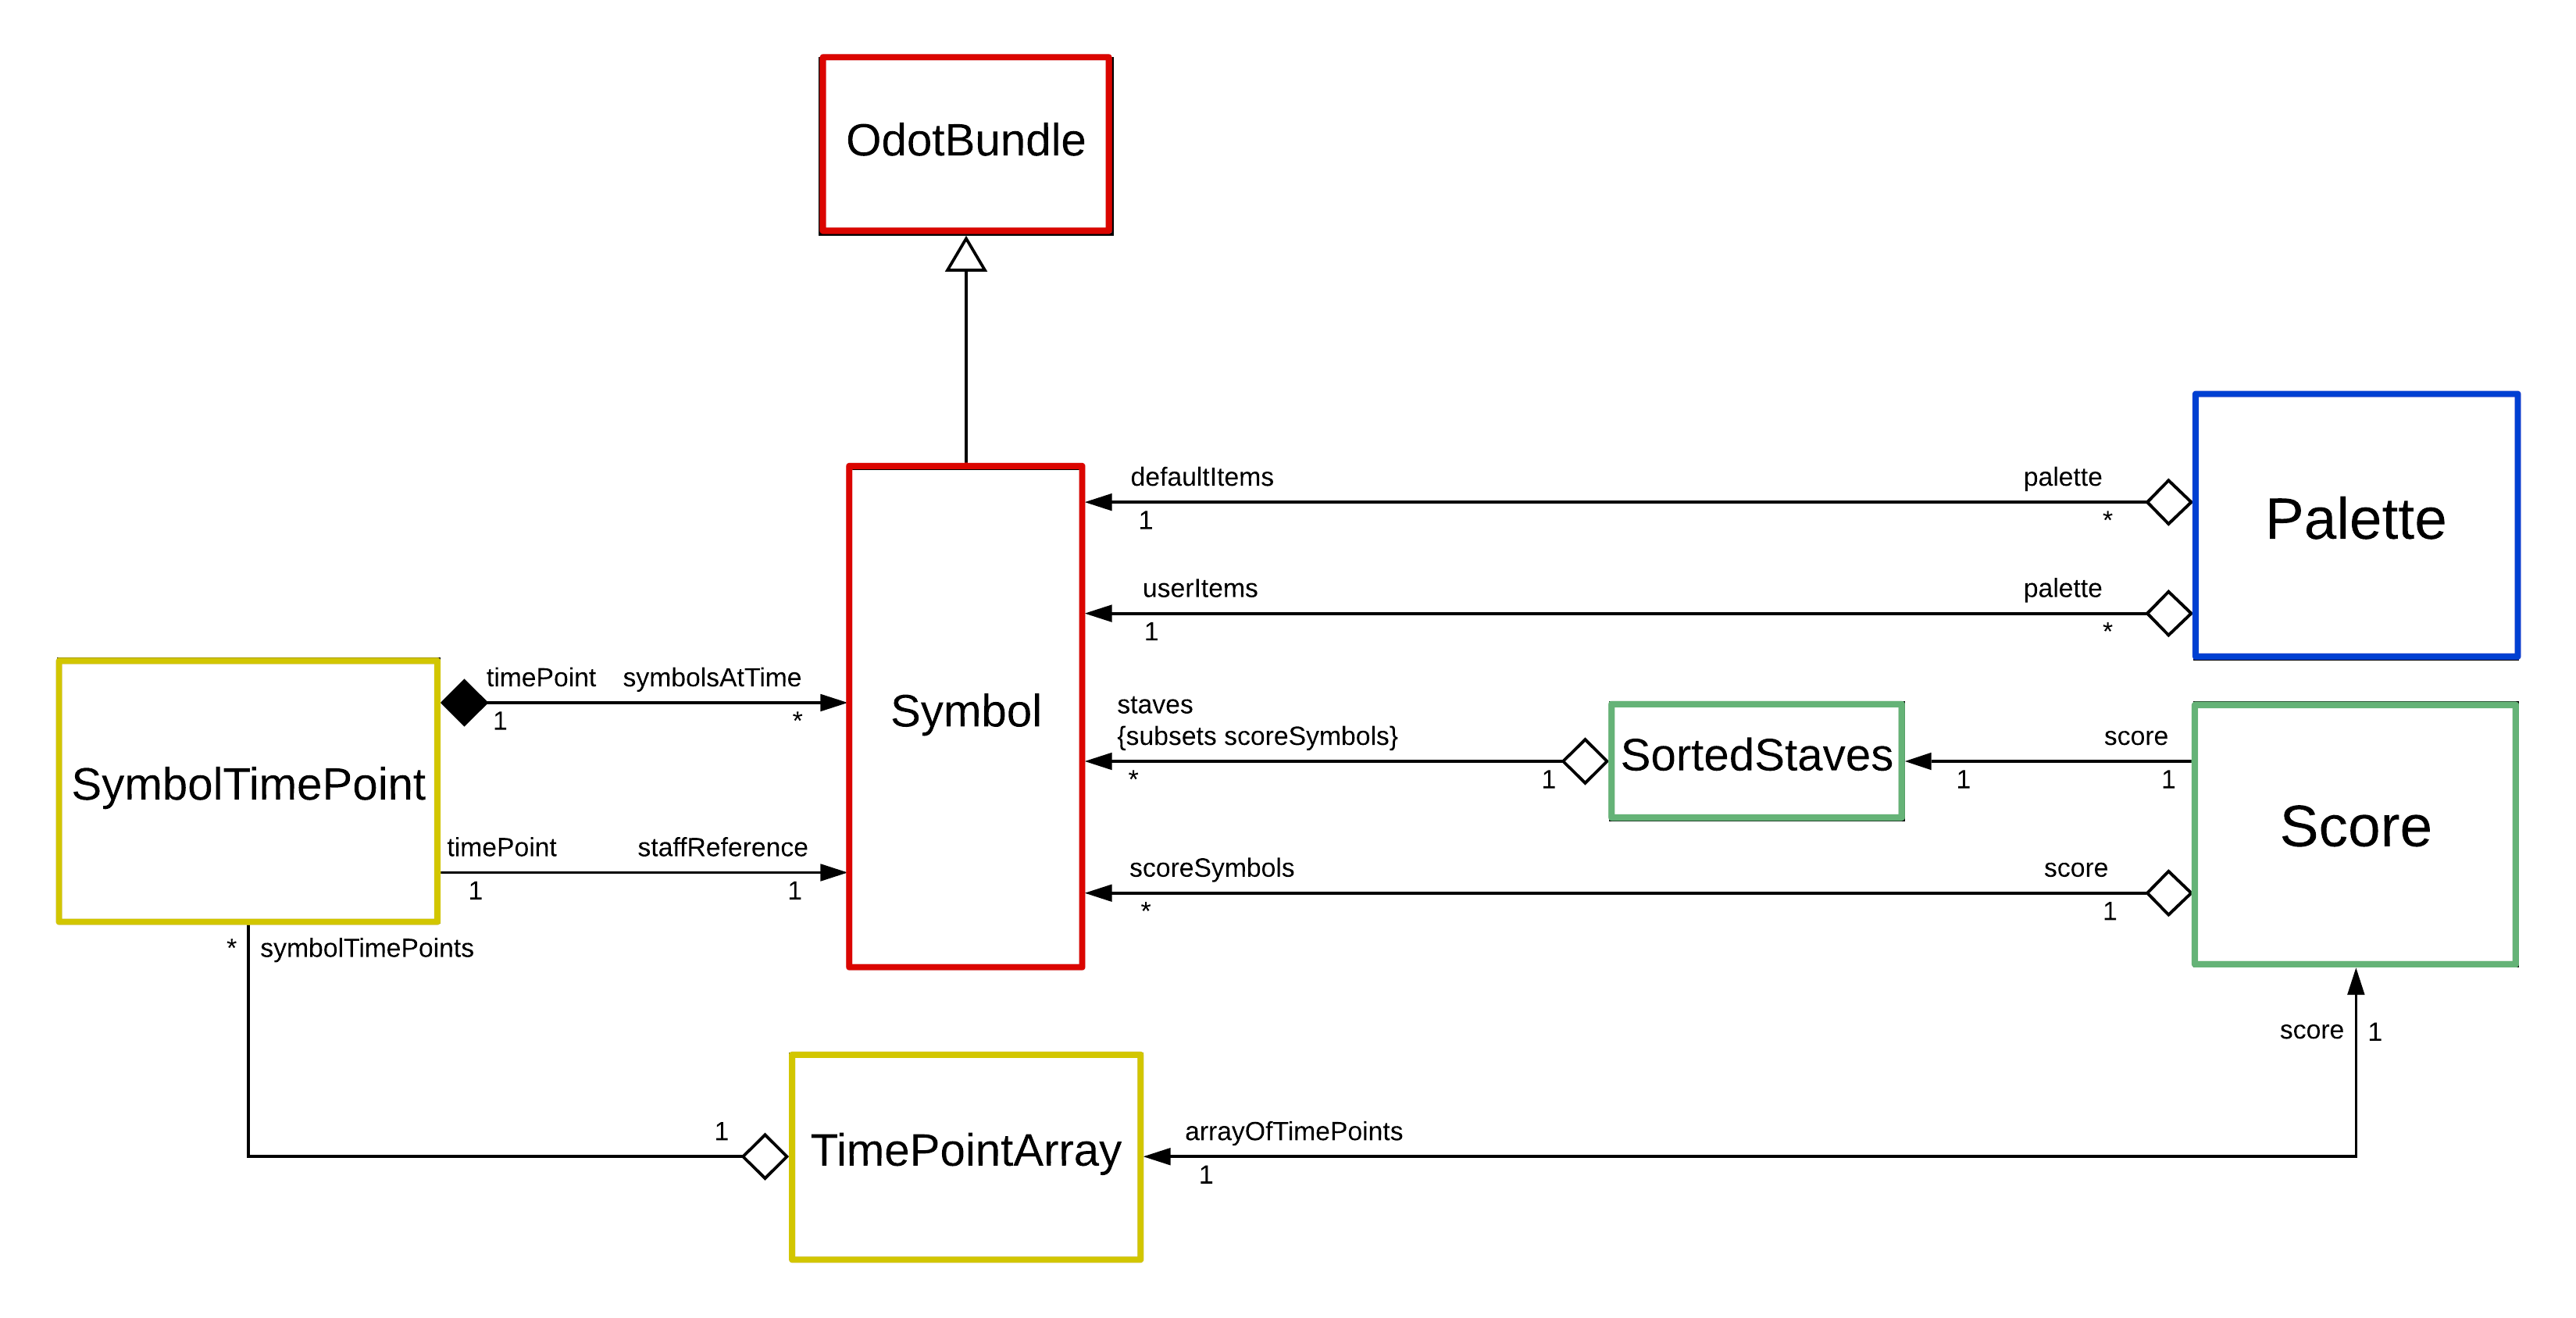
\includegraphics[keepaspectratio=true, width=\textwidth]{Annexes/i/symbolistModelClassDiagram.png}
		\captionof{figure}{Diagramme de classes pour le modèle de l'application symbolist}
		\label{fig:symbolistModelClassDiagram}	
		\medskip
		\small
		\it
		En \textcolor{red}{rouge}, la classe \emph{OdotBundle}, qui encapsule la structure d'un bundle \emph{OSC}, et la classe \emph{Symbol} dont les instances représentent les symboles de la partition. Chaque symbole de la partition possède une structure de bundle OSC, d'où la relation d'héritage entre la classe \emph{OdotBundle} et \emph{Symbol}.
		En \textcolor{blue}{bleu}, la classe \emph{Palette}, regroupant les symboles pouvant être dessinés sur la partition, qu'ils aient été définis par l'utilisateur ou existaient par défaut dans l'application.
		En \textcolor{green}{vert}, les classes \emph{Score} et \emph{SortedStaves} décrivant les symboles présent dans la partition.
		En \textcolor{yellow}{jaune}, les classes \emph{SymbolTimePoint} et \emph{TimePointArray} définissant la logique d'ordonnancement temporel des symboles associés à un \emph{staff}.  
	\end{minipage}
}
\clearpage

\rotatebox{90}{
	\begin{minipage}{0.85\textheight}
		\section{Architecture finale de l'application symbolist}
		\label{sec:symbolistFinalStructure}
		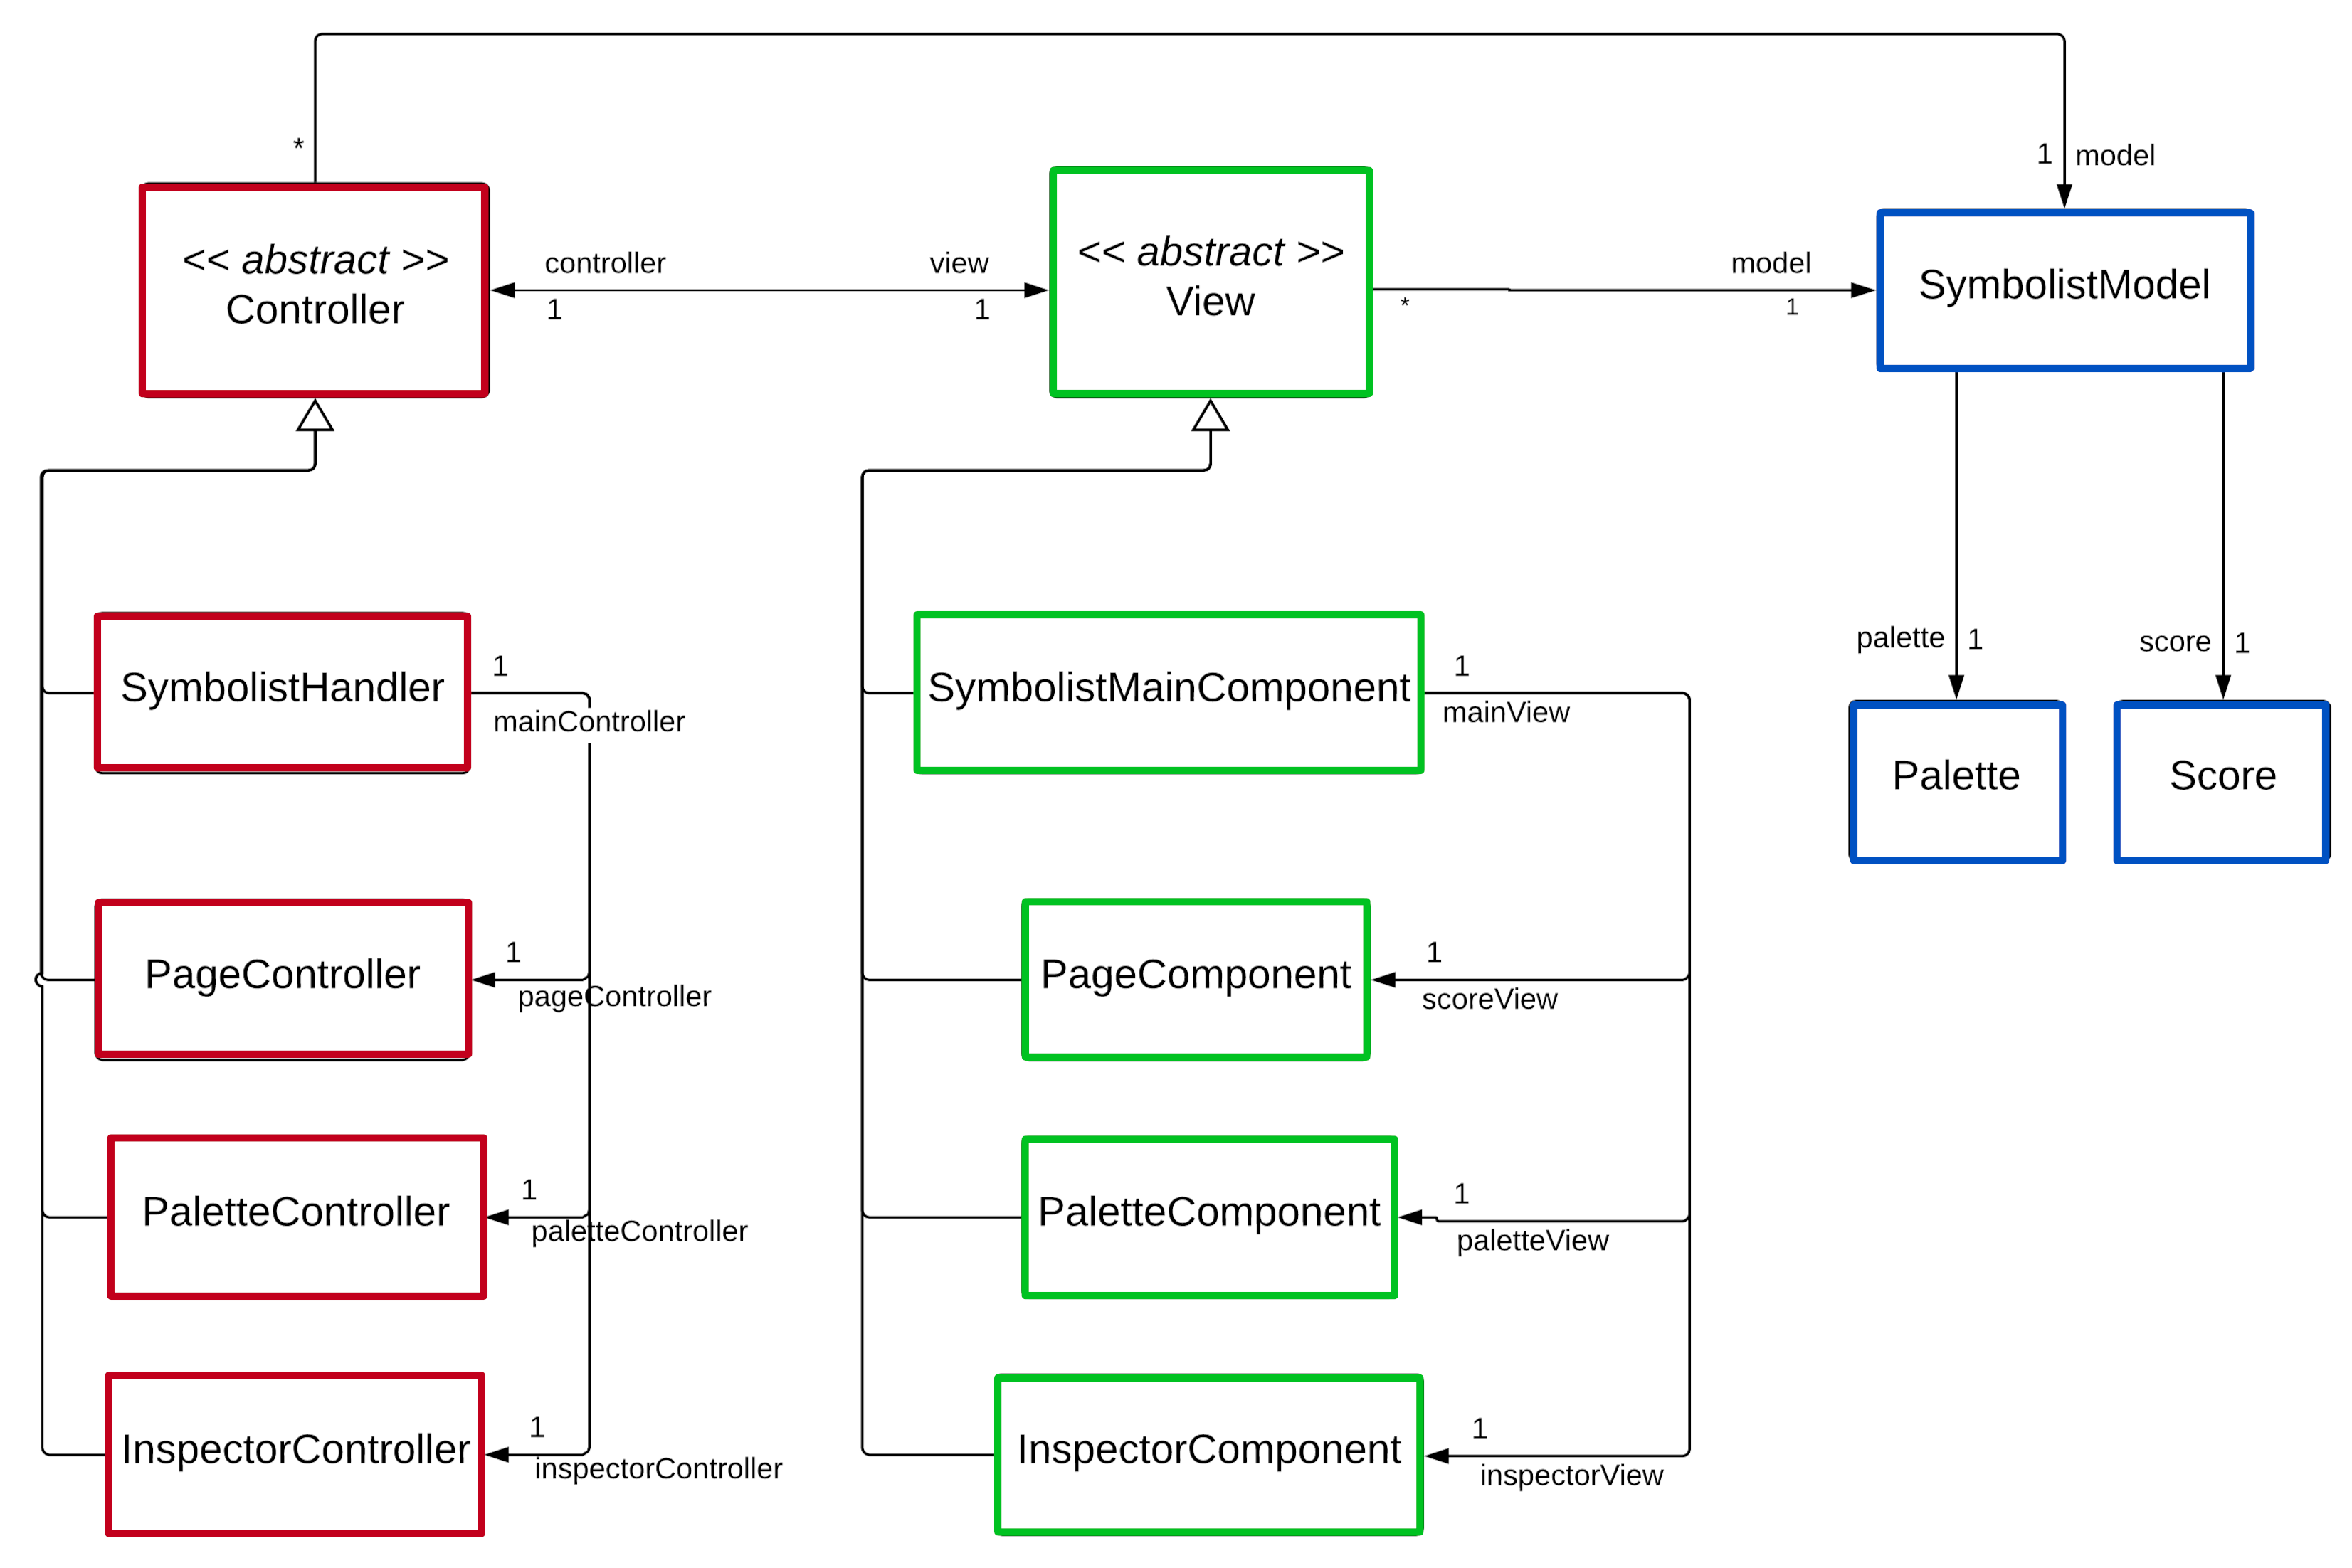
\includegraphics[keepaspectratio=true, width=\textwidth]{Annexes/i/symbolistFinalStructure.png}
		\captionof{figure}{Diagramme de classes présentant l'architecture de l'application symbolist après restructuration}
		\label{fig:symbolistFinalStructure}	
		\medskip
		\small
		\it
		En \textcolor{red}{rouge}, .
		En \textcolor{blue}{bleu}, .
		En \textcolor{green}{vert}, .  
	\end{minipage}
}
\clearpage
